\documentclass[aspectratio=169,10pt]{beamer}

\usepackage[T1]{fontenc}
\usepackage{lmodern}
\usepackage{amsmath,amssymb,booktabs,array}
\usepackage{tikz}
\usepackage{pgfpages}
\usepackage{pgfplots}
\usepackage{graphicx}
\usepackage{ragged2e}
\usepackage{appendixnumberbeamer}
\pgfplotsset{compat=1.15}

% Compile with \def\shownotes{1} to create a presenter-notes PDF.
\ifdefined\shownotes
  \setbeameroption{show notes on second screen=right}
\else
  \setbeameroption{hide notes}
\fi

\definecolor{Navy}{HTML}{102A43}
\definecolor{Blue}{HTML}{2F80ED}
\definecolor{Sky}{HTML}{D9EEFF}
\definecolor{Cyan}{HTML}{55C2FF}
\definecolor{Ink}{HTML}{172B4D}
\definecolor{Muted}{HTML}{5E6C84}
\definecolor{Panel}{HTML}{F1F4F8}
\definecolor{Green}{HTML}{2E8B57}
\definecolor{Orange}{HTML}{F2994A}
\definecolor{Red}{HTML}{D64545}
\definecolor{Teal}{HTML}{0EA5A8}
\definecolor{LightBlue}{HTML}{A9D6F5}

\usetheme{default}
\usefonttheme{professionalfonts}
\setbeamercolor{normal text}{fg=Ink,bg=white}
\setbeamercolor{frametitle}{fg=Navy,bg=white}
\setbeamercolor{structure}{fg=Blue}
\setbeamercolor{alerted text}{fg=Blue}
\setbeamercolor{block body}{fg=Ink,bg=Panel}
\setbeamercolor{alertblock body}{fg=Ink,bg=Sky}
\setbeamertemplate{navigation symbols}{}
\setbeamertemplate{itemize item}{\color{Blue}\raise0.2ex\hbox{\small$\blacktriangleright$}}
\setbeamertemplate{itemize subitem}{\color{Blue}\scriptsize$\bullet$}
\setbeamertemplate{frametitle}{%
  \vspace{0.35cm}\hspace{0.3cm}\insertframetitle\par
  \vspace{-0.12cm}\hspace{0.3cm}\color{Cyan}\rule{1.25cm}{1.5pt}}
\setbeamertemplate{footline}{%
  \leavevmode\hbox{%
  \begin{beamercolorbox}[wd=.82\paperwidth,ht=2.6ex,dp=1.1ex,leftskip=.45cm]{author in head/foot}%
    \color{Muted}\scriptsize Erd\H{o}s Institute Quantitative Finance Project
  \end{beamercolorbox}%
  \begin{beamercolorbox}[wd=.18\paperwidth,ht=2.6ex,dp=1.1ex,rightskip=.45cm plus1fil]{date in head/foot}%
    \color{Muted}\scriptsize \insertframenumber/\inserttotalframenumber
  \end{beamercolorbox}}}
\setbeamerfont{frametitle}{size=\Large,series=\bfseries}
\setbeamerfont{title}{size=\fontsize{27}{31}\selectfont,series=\bfseries}
\setbeamerfont{subtitle}{size=\large}

\newcommand{\tagline}[1]{\textcolor{Blue}{\bfseries\scriptsize\MakeUppercase{#1}}}
\newcommand{\metric}[3]{%
\begin{beamercolorbox}[rounded=true,sep=0.22cm,wd=\linewidth]{block body}
  {\color{#3}\fontsize{20}{22}\selectfont\bfseries #1}\par
  \vspace{0.08cm}{\small #2}
\end{beamercolorbox}}

\title{Can Market Signals Improve Delta Hedging?}
\subtitle{A leakage-controlled replication experiment on historical SPY paths}
\author{Yue Wu \and Freda Zhang}
\institute{The Erd\H{o}s Institute -- Quantitative Finance}
\date{Summer 2026}

\begin{document}

% 1
\begin{frame}[plain]
\begin{tikzpicture}[remember picture,overlay]
  \fill[Navy] (current page.south west) rectangle (current page.north east);
  \fill[Blue] ([xshift=-1.1cm]current page.north east) rectangle (current page.north east);
  \fill[Cyan] ([xshift=-1.1cm,yshift=-2.2cm]current page.north east) rectangle ([yshift=-2.2cm]current page.north east);
\end{tikzpicture}
\vspace{0.65cm}
{\color{Cyan}\tagline{Erd\H{o}s Institute -- Summer 2026}}\par
\vspace{1.0cm}
{\color{white}\usebeamerfont{title}\inserttitle}\par
\vspace{0.35cm}
{\color{Sky}\usebeamerfont{subtitle}\insertsubtitle}\par
\vfill
{\color{white}\large Yue Wu \quad Freda Zhang}\par
\vspace{0.15cm}{\color{Sky}\small Quantitative Finance Project}
\note{Hi everyone. Today we will share our quantitative finance project on whether public market signals can improve delta hedging. In our leakage-controlled experiment on historical SPY paths, VIX reduces the largest hedging losses, while our more complex composite signal does not improve average accuracy.}
\end{frame}

% 2
\begin{frame}{We test hedge inputs -- not historical option execution}
\begin{columns}[T,onlytextwidth]
\column{0.46\textwidth}
\vspace{0.4cm}
{\fontsize{19}{23}\selectfont\bfseries Can point-in-time signals reduce terminal replication error versus fixed-volatility Black--Scholes?}

\vspace{0.55cm}
\begin{beamercolorbox}[rounded=true,sep=0.3cm]{block body}
\textbf{Controlled comparison}\par
Same payoff, initial premium, hedge calendar, and transaction-cost rule.
\end{beamercolorbox}

\column{0.49\textwidth}
\tagline{Observed market data}
\begin{itemize}
  \item SPY adjusted prices and volume
  \item VIX, XLK returns, and short rates
\end{itemize}
\vspace{0.25cm}
\tagline{Model-defined claims}
\begin{itemize}
  \item European calls with controlled maturity and moneyness
  \item No historical option bids, asks, or contract IV
\end{itemize}
\end{columns}
\note{First, the scope: prices, volume, VIX, sector returns, and rates are real point-in-time observations. The options are standardized European calls placed on those paths; we do not use historical option quotes. Holding payoff, premium, hedge dates, and costs fixed lets us isolate the volatility input.}
\end{frame}

% 3
\begin{frame}{Four strategies; one common delta engine}
\small
\begin{columns}[T,onlytextwidth]
\column{0.235\textwidth}
\begin{beamercolorbox}[rounded=true,sep=0.28cm]{block body}
\tagline{FV-BS}\par\vspace{0.15cm}
\textbf{Fixed 21-day realized volatility}\par\vspace{0.25cm}
Benchmark fixed at contract initiation.
\end{beamercolorbox}
\column{0.235\textwidth}
\begin{beamercolorbox}[rounded=true,sep=0.28cm]{block body}
\tagline{Rolling-BS}\par\vspace{0.15cm}
\textbf{Updated 21-day realized volatility}\par\vspace{0.25cm}
Uses the latest price information.
\end{beamercolorbox}
\column{0.235\textwidth}
\begin{beamercolorbox}[rounded=true,sep=0.28cm]{alertblock body}
\tagline{VIX-BS}\par\vspace{0.15cm}
\textbf{Daily VIX as hedge volatility}\par\vspace{0.25cm}
Adds forward-looking option-market information.
\end{beamercolorbox}
\column{0.235\textwidth}
\begin{beamercolorbox}[rounded=true,sep=0.28cm]{block body}
\tagline{MSA-Delta}\par\vspace{0.15cm}
\textbf{Rolling vol $\times$ risk multiplier}\par\vspace{0.25cm}
Combines seven market signals.
\end{beamercolorbox}
\end{columns}
\vspace{0.55cm}
\centering
\colorbox{Sky}{\parbox{0.88\textwidth}{\centering\textbf{Common premium $\cdot$ daily rebalancing $\cdot$ identical payoff $\cdot$ identical costs}}}
\note{The four strategies share one Black--Scholes delta engine. FV-BS freezes 21-day realized volatility; Rolling-BS updates it daily; VIX-BS uses daily VIX; and MSA-Delta adjusts rolling volatility with seven signals. Everything else is identical, so differences come from the volatility input.}
\end{frame}

% 4
\begin{frame}{Definition: volatility changes delta away from the money}
\begin{columns}[T,onlytextwidth]
\column{0.49\textwidth}
\tagline{Common hedge formula}
\begin{beamercolorbox}[rounded=true,sep=0.32cm]{block body}
\scriptsize
\[
\Delta_t=N(d_{1,t}),\qquad
d_{1,t}=\frac{\ln(S_t/K)+(r+\tfrac12\sigma_t^2)\tau}
{\sigma_t\sqrt{\tau}}.
\]
\end{beamercolorbox}
\vspace{0.35cm}
\textbf{Example contract}\par
$S=100$, $K=105$, $\tau=21/252$, and $r=3\%$.

\column{0.47\textwidth}
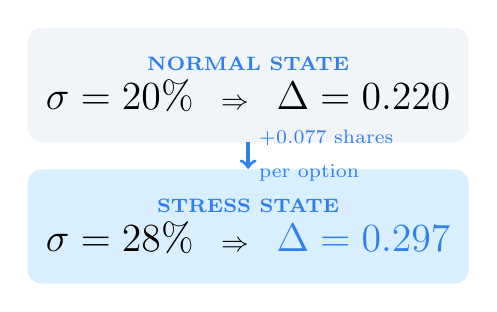
\begin{tikzpicture}
\node[rounded corners=5pt,fill=Panel,minimum width=5.6cm,minimum height=1.45cm,align=center] (a) at (0,1.15) {\tagline{Normal state}\\[2pt]{\Large$\sigma=20\%$}\quad$\Rightarrow$\quad{\Large$\Delta=0.220$}};
\node[rounded corners=5pt,fill=Sky,minimum width=5.6cm,minimum height=1.45cm,align=center] (b) at (0,-0.65) {\tagline{Stress state}\\[2pt]{\Large$\sigma=28\%$}\quad$\Rightarrow$\quad{\color{Blue}\Large$\Delta=0.297$}};
\draw[->,very thick,Blue] (a.south) -- (b.north) node[midway,right,align=left] {\scriptsize $+0.077$ shares\\\scriptsize per option};
\end{tikzpicture}
\end{columns}
\vspace{0.2cm}
\begin{beamercolorbox}[rounded=true,sep=0.22cm]{alertblock body}
\textbf{Why this matters:} volatility adjustments materially change OTM and ITM deltas, but have little effect on an ATM delta near $0.5$.
\end{beamercolorbox}
\note{Why does the input matter? In this out-of-the-money example, raising volatility from 20 to 28 percent raises delta from 0.220 to 0.297---about eight additional shares per hundred options. The effect is strongest away from the money; at-the-money delta remains near one-half.}
\end{frame}

% 5
\begin{frame}{Definition: seven trailing signals create three risk states}
\begin{columns}[T,onlytextwidth]
\column{0.57\textwidth}
\tagline{Standardized risk score}
\begin{beamercolorbox}[rounded=true,sep=0.25cm]{block body}
\scriptsize
\begin{align*}
R_t={}&0.30\,\mathrm{IVRank}_t+0.20\,\mathrm{VIX}_t
+0.20\,\frac{\mathrm{RV}_{21,t}}{\mathrm{RV}_{63,t}}\\
&+0.10\,\mathrm{VolumeShock}_t
+0.10\,\mathrm{Drawdown}_{63,t}\\
&+0.05\,\mathrm{SectorDiv}_t
+0.05\,|\Delta\mathrm{Rate}_{21,t}|.
\end{align*}
\end{beamercolorbox}
\vspace{0.25cm}
\small Features are standardized using development-period statistics only.

\column{0.39\textwidth}
\begin{beamercolorbox}[rounded=true,sep=0.25cm]{block body}
\tagline{Normal}\quad $R_t<q_{70}$\hfill $m=1.00$
\end{beamercolorbox}
\vspace{0.22cm}
\begin{beamercolorbox}[rounded=true,sep=0.25cm]{alertblock body}
\tagline{Elevated}\quad $q_{70}\le R_t<q_{90}$\hfill $m=1.15$
\end{beamercolorbox}
\vspace{0.22cm}
\begin{beamercolorbox}[rounded=true,sep=0.25cm]{alertblock body}
\tagline{Stress}\quad $R_t\ge q_{90}$\hfill $m=1.40$
\end{beamercolorbox}
\vspace{0.35cm}
\centering$\sigma_t^{\mathrm{MSA}}=m(Z_t)\widehat\sigma_{21,t}$
\end{columns}
\note{Our composite score combines seven trailing indicators, led by VIX rank, VIX level, and the realized-volatility ratio. Development-period statistics standardize the features. The score maps to normal, elevated, or stress multipliers of 1, 1.15, and 1.4. Every day-$t$ input was observable on day $t$.}
\end{frame}

% 6
\begin{frame}{The test period stays untouched until final evaluation}
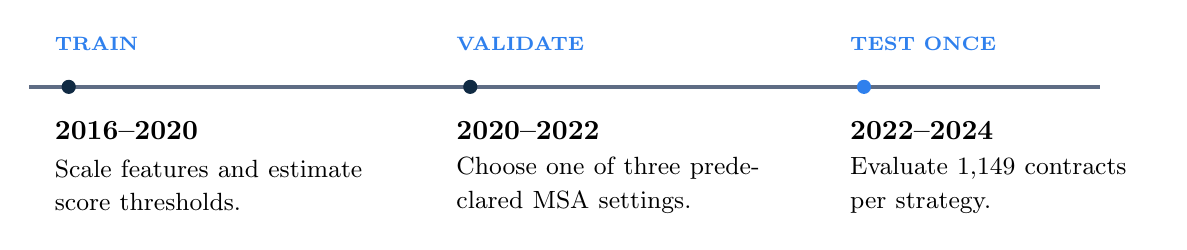
\begin{tikzpicture}[x=1cm,y=1cm]
\draw[very thick,Muted] (0.7,2.65) -- (14.3,2.65);
\foreach \x/\c in {1.2/Navy,6.3/Navy,11.3/Blue}{\fill[\c] (\x,2.65) circle (0.09);}
\node[anchor=west] at (0.9,3.2) {\tagline{Train}};
\node[anchor=west] at (0.9,2.1) {\textbf{2016--2020}};
\node[anchor=west,text width=4.0cm] at (0.9,1.4) {\small Scale features and estimate score thresholds.};
\node[anchor=west] at (6.0,3.2) {\tagline{Validate}};
\node[anchor=west] at (6.0,2.1) {\textbf{2020--2022}};
\node[anchor=west,text width=4.0cm] at (6.0,1.4) {\small Choose one of three predeclared MSA settings.};
\node[anchor=west,text=Blue] at (11.0,3.2) {\tagline{Test once}};
\node[anchor=west] at (11.0,2.1) {\textbf{2022--2024}};
\node[anchor=west,text width=3.8cm] at (11.0,1.4) {\small Evaluate 1,149 contracts per strategy.};
\end{tikzpicture}
\vspace{-0.25cm}
\begin{columns}[onlytextwidth]
\column{0.32\textwidth}\metric{3}{maturities: 10, 21, 42 days}{Blue}
\column{0.32\textwidth}\metric{3}{strike/spot: 0.95, 1.00, 1.05}{Navy}
\column{0.32\textwidth}\metric{5}{trading days between starts}{Navy}
\end{columns}
\note{This split protects against leakage. We fit scaling and thresholds in 2016--2020, select one predeclared setting in 2020--2022, and evaluate once on untouched 2022--2024 data. Three maturities and three moneyness levels, starting every five days, produce 1,149 contracts per strategy.}
\end{frame}

% 7
\begin{frame}{No single hedge wins every error metric}
\begin{columns}[T,onlytextwidth]
\column{0.66\textwidth}
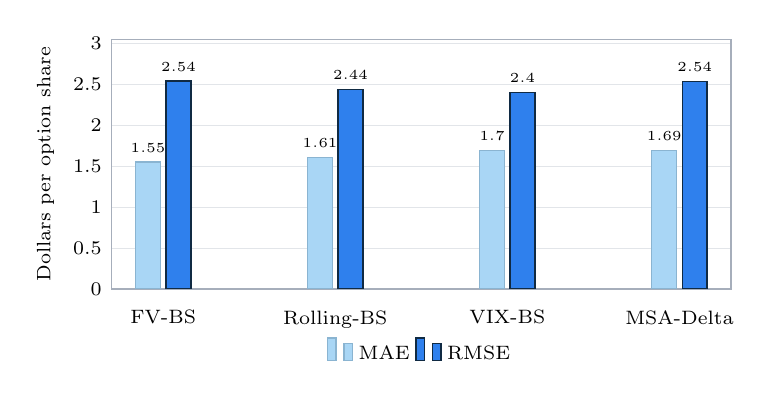
\begin{tikzpicture}
\begin{axis}[
  ybar,bar width=9pt,width=9.45cm,height=4.75cm,
  ymin=0,ymax=3.05,ytick={0,0.5,...,3},
  symbolic x coords={FV-BS,Rolling-BS,VIX-BS,MSA-Delta},xtick=data,
  tick label style={font=\scriptsize},
  legend style={at={(0.5,-0.17)},anchor=north,legend columns=2,font=\scriptsize,draw=none},
  ymajorgrids,grid style={draw=Muted!18,line width=.35pt},axis line style={draw=Muted!55,line width=.6pt},
  tick style={draw=none},
  ylabel={Dollars per option share},ylabel style={font=\scriptsize}]
\addplot[fill=LightBlue,draw=LightBlue!80!Navy,line width=.5pt,nodes near coords={\pgfmathprintnumber[fixed,precision=2]{\pgfplotspointmeta}},nodes near coords style={font=\tiny,anchor=south},point meta=y] coordinates {(FV-BS,1.5523) (Rolling-BS,1.6074) (VIX-BS,1.6956) (MSA-Delta,1.6906)};
\addplot[fill=Blue,draw=Navy,line width=.5pt,nodes near coords={\pgfmathprintnumber[fixed,precision=2]{\pgfplotspointmeta}},nodes near coords style={font=\tiny,anchor=south},point meta=y] coordinates {(FV-BS,2.5422) (Rolling-BS,2.4385) (VIX-BS,2.3993) (MSA-Delta,2.5368)};
\legend{MAE,RMSE}
\end{axis}
\end{tikzpicture}

\column{0.31\textwidth}
\metric{1.552}{Lowest MAE: FV-BS}{Navy}
\vspace{0.3cm}
\metric{2.399}{Lowest RMSE: VIX-BS}{Blue}
\vspace{0.45cm}
\small\textbf{Interpretation}\par
Average accuracy favors simplicity; large-error control favors forward-looking volatility.
\end{columns}
\note{Here are the headline test results; lower is better. FV-BS has the lowest MAE at 1.552, so it wins on average absolute accuracy. VIX-BS has the lowest RMSE at 2.399, meaning it better controls large errors. MSA-Delta wins neither metric.}
\end{frame}

% 8
\begin{frame}{VIX helps most where losses are largest}
\begin{columns}[T,onlytextwidth]
\column{0.31\textwidth}
\metric{5.52}{VIX-BS 95\% loss Expected Shortfall}{Blue}
\vspace{0.35cm}
\metric{6.75}{FV-BS 95\% loss Expected Shortfall}{Navy}
\vspace{0.45cm}
\small Lower is better. VIX reduces expected loss in the worst 5\% of outcomes by about \textbf{18\%}.

\column{0.65\textwidth}
\tagline{Paired MAE improvement over FV-BS}
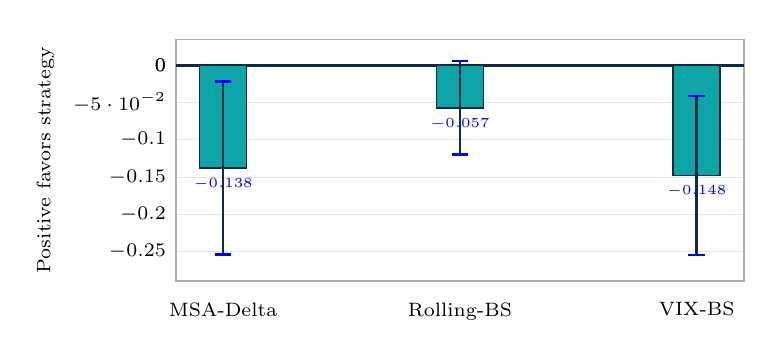
\begin{tikzpicture}
\begin{axis}[
  ybar,width=8.8cm,height=4.65cm,bar width=17pt,
  ymin=-0.29,ymax=0.035,ytick={-0.25,-0.20,...,0},
  symbolic x coords={MSA-Delta,Rolling-BS,VIX-BS},xtick=data,
  tick label style={font=\scriptsize},
  ymajorgrids,grid style={draw=Muted!18,line width=.35pt},axis line style={draw=Muted!55,line width=.6pt},
  tick style={draw=none},
  extra y ticks={0},extra y tick style={grid=major,grid style={draw=Navy,very thick}},
  ylabel={Positive favors strategy},ylabel style={font=\scriptsize}]
\addplot+[fill=Teal,draw=Navy,line width=.6pt,nodes near coords={\pgfmathprintnumber[fixed,precision=3]{\pgfplotspointmeta}},nodes near coords style={font=\tiny,anchor=north},point meta=y,error bars/.cd,y dir=both,y explicit,error bar style={line width=1pt,draw=Navy},error mark options={rotate=90,mark size=3pt,line width=1pt}]
coordinates {(MSA-Delta,-0.138) +- (0,0.116) (Rolling-BS,-0.057) +- (0,0.063) (VIX-BS,-0.148) +- (0,0.107)};
\end{axis}
\end{tikzpicture}
\centering\scriptsize 95\% moving date-block bootstrap intervals
\end{columns}
\note{The benefit appears in the loss tail. In the worst five percent of outcomes, VIX-BS reduces expected loss from 6.75 to 5.52 dollars---about 18 percent. But every MAE-improvement estimate is below zero; the bootstrap intervals show no average-error advantage for VIX or MSA. VIX helps severe losses, not typical absolute error.}
\end{frame}

% 9
\begin{frame}{The ranking survives transaction-cost changes}
\centering
\renewcommand{\arraystretch}{1.45}
\begin{tabular}{>{\bfseries}lcc}
\toprule
Transaction cost & Lowest MAE & Lowest RMSE \\
\midrule
0 bps  & FV-BS \; 1.456 & \textcolor{Blue}{VIX-BS \; 2.394} \\
5 bps  & FV-BS \; 1.552 & \textcolor{Blue}{VIX-BS \; 2.399} \\
10 bps & FV-BS \; 1.745 & \textcolor{Blue}{VIX-BS \; 2.510} \\
\bottomrule
\end{tabular}
\vspace{0.65cm}
\begin{columns}[onlytextwidth]
\column{0.48\textwidth}
\begin{beamercolorbox}[rounded=true,sep=0.28cm]{block body}
\tagline{Stable finding 1}\par
Fixed volatility remains best for average absolute error.
\end{beamercolorbox}
\column{0.48\textwidth}
\begin{beamercolorbox}[rounded=true,sep=0.28cm]{alertblock body}
\tagline{Stable finding 2}\par
VIX remains best for squared error at every cost level.
\end{beamercolorbox}
\end{columns}
\vspace{0.35cm}
\scriptsize Results are also reported for all nine maturity--moneyness cells.
\note{The ranking is stable at zero, five, and ten basis points: FV-BS retains the lowest MAE, while VIX-BS retains the lowest RMSE. Winners vary across individual maturity and moneyness cells, so no method dominates every contract and objective.}
\end{frame}

% 10
\begin{frame}{The useful signal is simpler than the model we designed}
\vspace{0.2cm}
{\fontsize{19}{23}\selectfont\bfseries Forward-looking volatility improves tail-risk control -- but more signals do not guarantee a better hedge.}
\vspace{0.6cm}
\begin{columns}[T,onlytextwidth]
\column{0.31\textwidth}
\begin{beamercolorbox}[rounded=true,sep=0.3cm]{alertblock body}
\tagline{Keep}\par\vspace{0.12cm}
\textbf{VIX-BS} as the strongest tail-risk benchmark.
\end{beamercolorbox}
\column{0.31\textwidth}
\begin{beamercolorbox}[rounded=true,sep=0.3cm]{block body}
\tagline{Reject}\par\vspace{0.12cm}
A blanket claim that additional complexity improves hedging.
\end{beamercolorbox}
\column{0.31\textwidth}
\begin{beamercolorbox}[rounded=true,sep=0.3cm]{block body}
\tagline{Next}\par\vspace{0.12cm}
Repeat the design using contract-level option quotes when available.
\end{beamercolorbox}
\end{columns}
\vspace{0.55cm}
\tagline{Important limitations}
\begin{itemize}
  \item VIX is an index-level 30-day proxy, not contract-level SPY IV.
  \item Controlled European claims omit historical spreads and early exercise.
  \item Block bootstrap mitigates, but does not eliminate, overlap dependence.
\end{itemize}
\note{Our conclusion is simple: keep VIX-BS as a strong tail-risk benchmark, but reject the claim that more signals automatically improve hedging. The main limits are VIX as a proxy, standardized European claims, and overlapping contracts. Next, we would repeat the design with contract-level option quotes. Thank you---we welcome your questions.}
\end{frame}

\end{document}
